A business canvas gives an overview of a company's business model.
Based on our analysis we have the following understanding of Valcon's canvas (see figure \ref{fig:canvas}).

\begin{figure}[!htp]
\centering
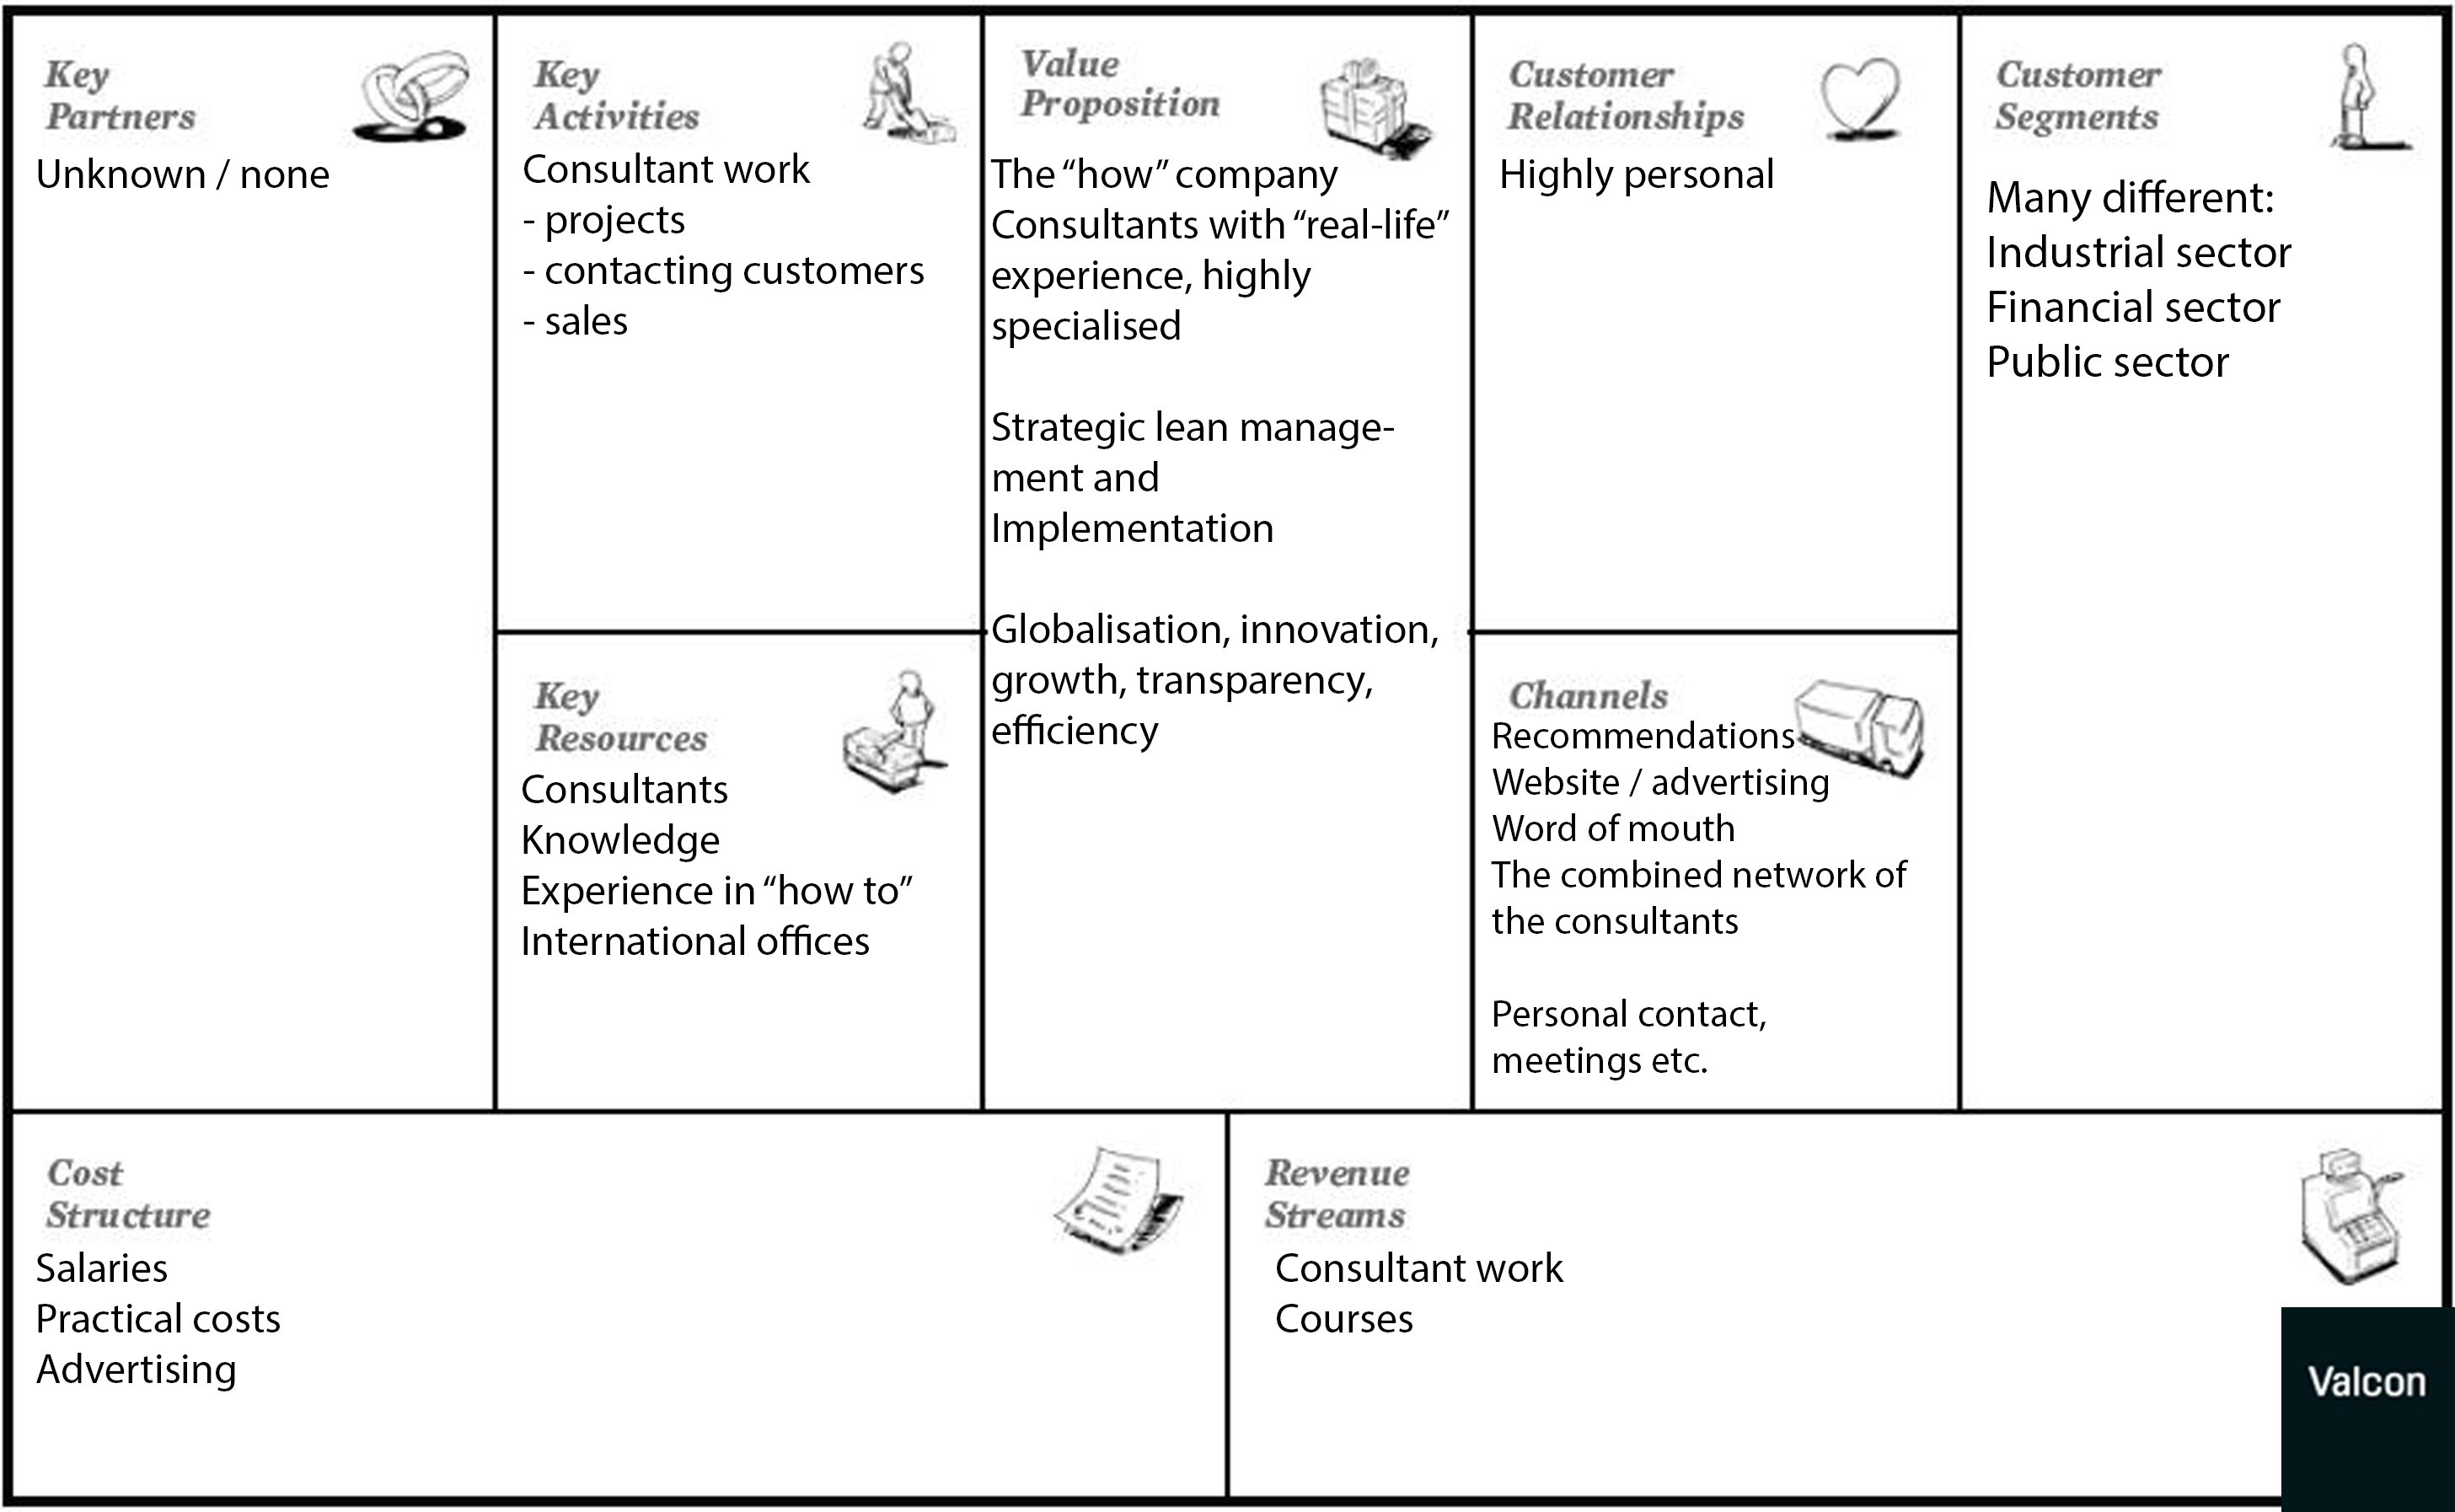
\includegraphics[width=\textwidth]{inline/business-model-canvas.png}
\caption{Valcon's business canvas.}
\label{fig:canvas}
\end{figure}

In relation to the problem it is important to note that the consultants are key resources, as they are the ones who generate revenue.
As such it is important that they are able to perform their work effectively as soon as they start working at Valcon. This gives us an understanding of why the company might value the consultants' time highly. (Source: Valcon's homepage. Approved by Danni during inline conclusion meeting (appendix \ref{app:danni_inline}).) 
For a larger version of the canvas See appendix \ref{app:canvas}.